\section{Auswertung}
\label{sec:Auswertung}

\subsection{Fouriesynthese}
Im ersten Teil des Experiments wurden wie in der Durchführung beschrieben die Spannungsverläufe zusammengesetzt. 

In Abbildung (\ref{fig:plot1}) ist die Fouriereihe der Sägezahnspannung zu sehen.
\begin{figure}[H]
  \centering
  \includegraphics[width = 0.7\linewidth]{Sägezahn.jpeg}
  \caption{Verlauf der Sägezahnspannung.}
  \label{fig:plot1}
\end{figure}

In Abbildung (\ref{fig:plot2}) ist die Fouriereihe der Dreiecksspannung zu erkennen. 
\begin{figure}[H]
  \centering
  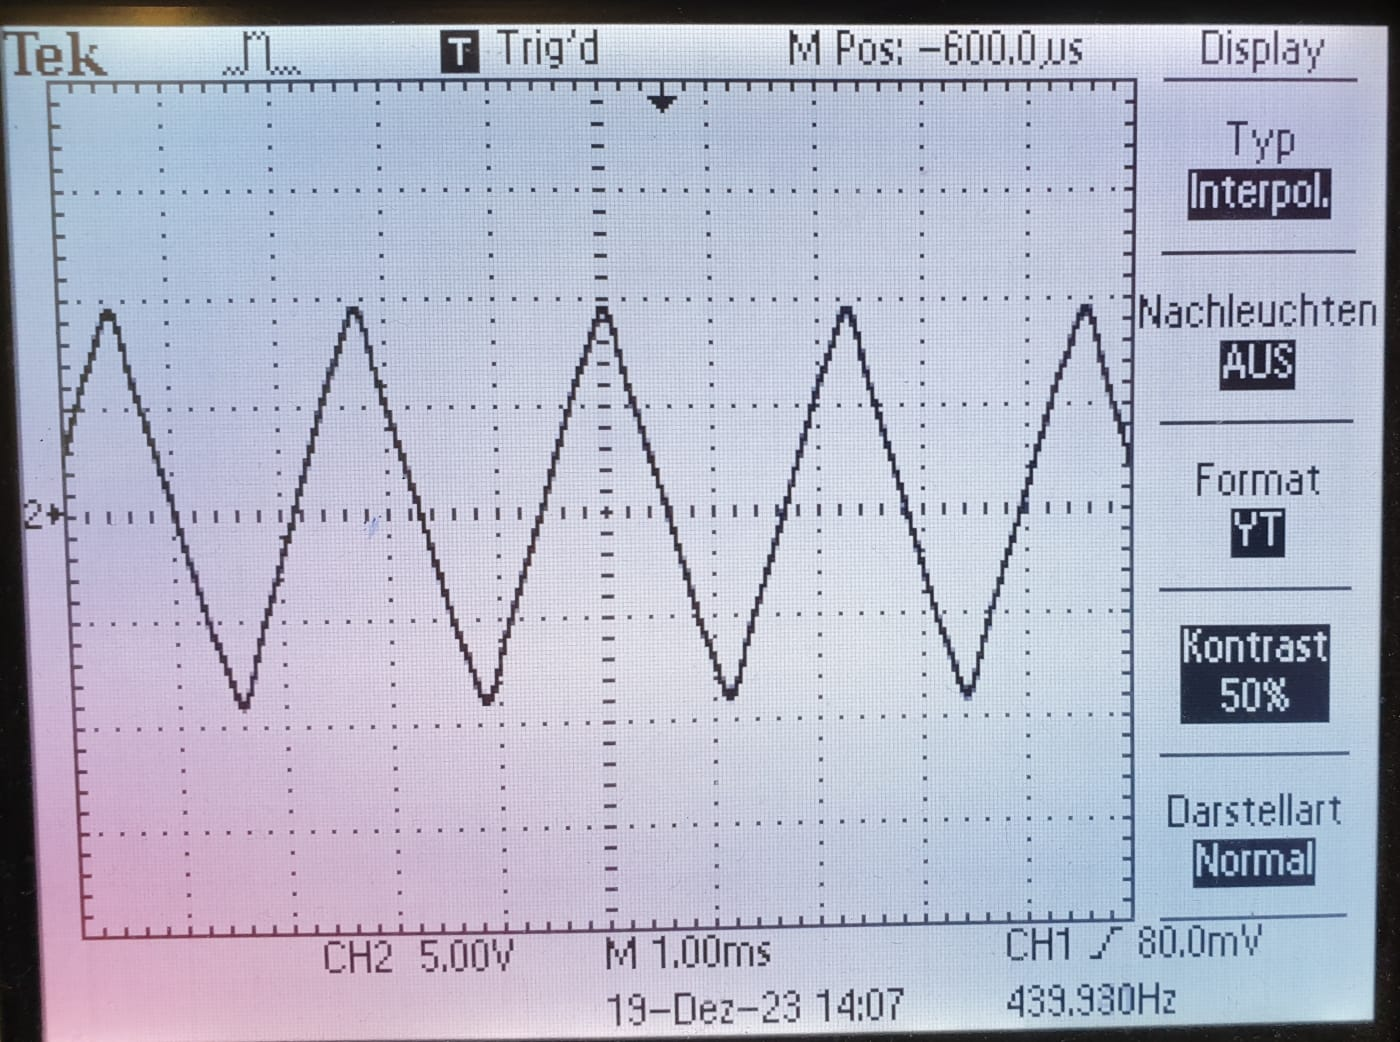
\includegraphics[width = 0.7\linewidth]{Dreieck.jpeg}
  \caption{Verlauf der Dreiecksspannung.}
  \label{fig:plot2}
\end{figure}

Außerdem ist in Abbildung (\ref{fig:plot3}) die Fouriereihe der Rechteckspannung
\begin{figure}[H]
  \centering
  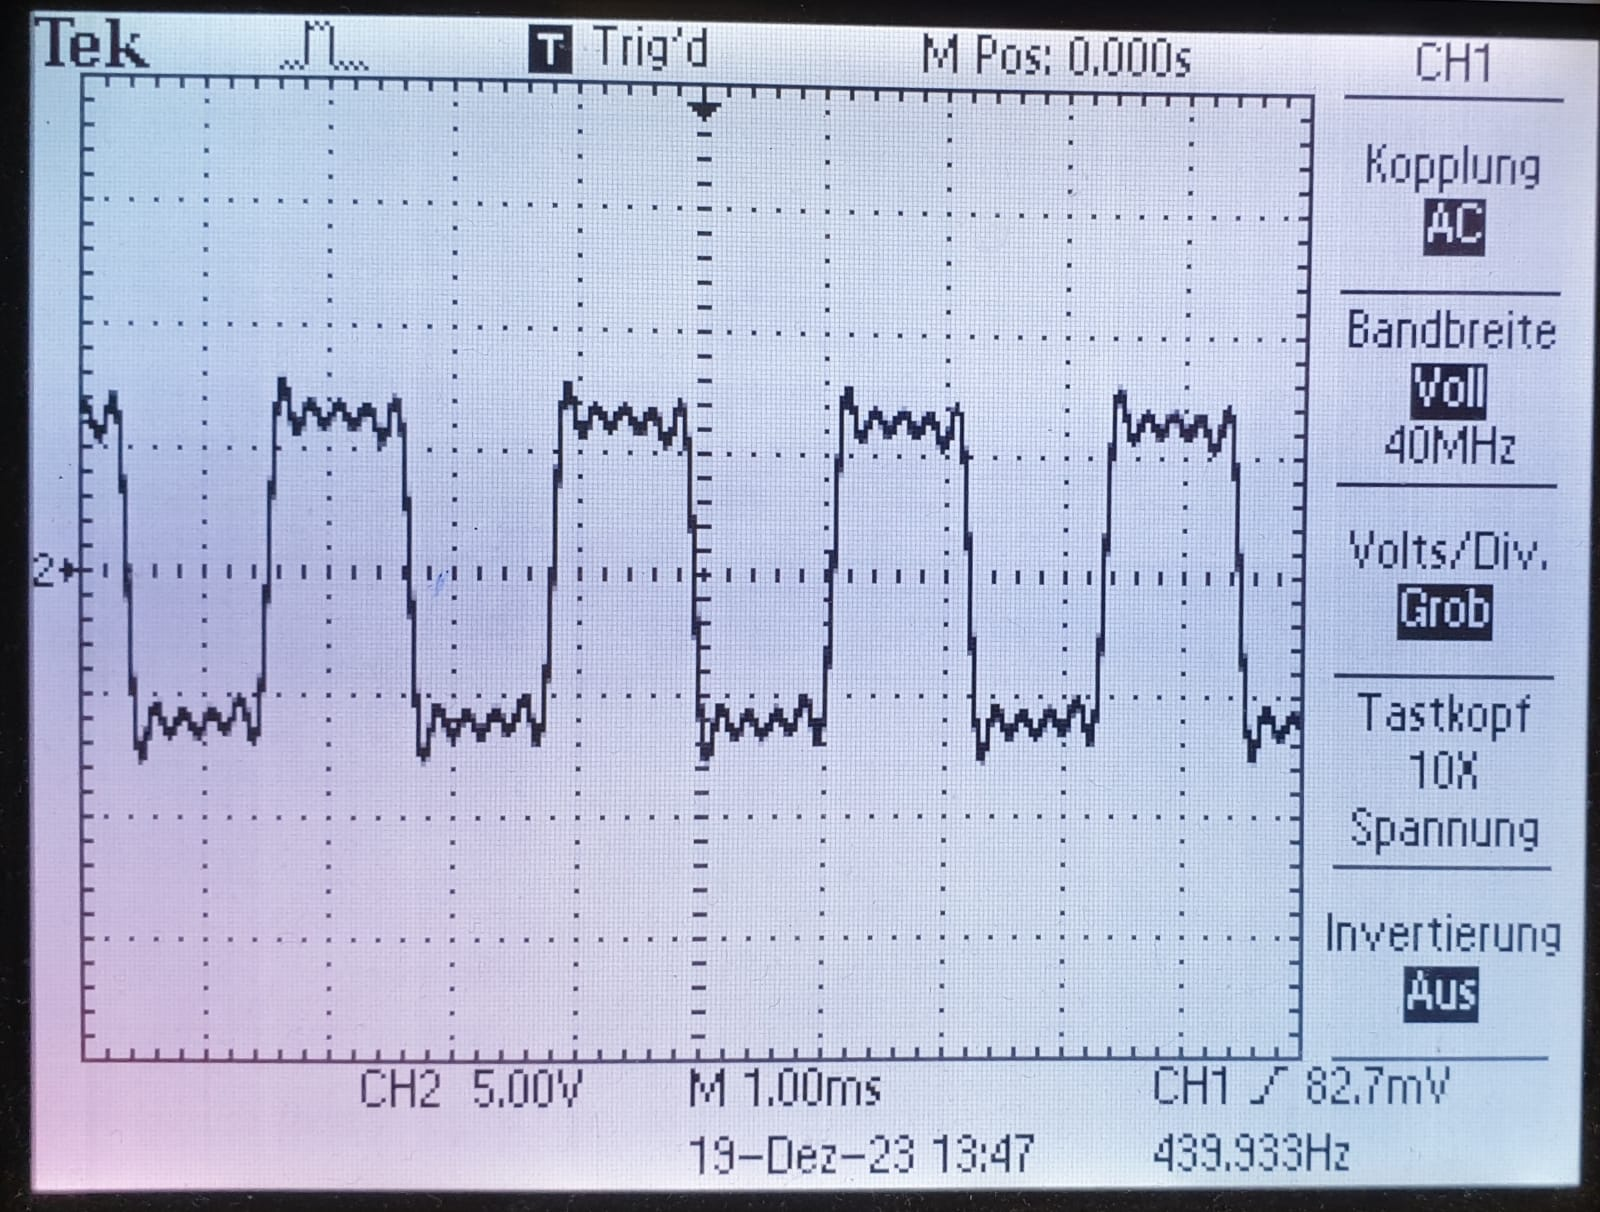
\includegraphics[width = 0.7\linewidth]{Viereck.jpeg}
  \caption{Verlauf der Rechteckspannung.}
  \label{fig:plot2}
\end{figure}

\subsection{Fourieanalyse}
Im zweiten Teil des Experiments wurde das Linienspektrums der Sägezahnspannung, Dreiecksspannung und Rechteckspannung auf dem Oszilloskop eingestellt, um dann 
mithilfe des Cursers die Höhe der Peaks messen zu können. \\
\textbf{Sägezahnspannung} \\
Die Frequenz wird in Kilohertz und die Höhe der Peaks wird in Dezibil gemessen. Die aufgenommenen Messdaten sind in Tabelle (\ref{tab:saegezahn}) aufgeführt. 
\textbf{Dreiecksspannung} \\
\textbf{Rechteckspannung} \\





%Siehe \autoref{fig:plot}!